\section{商业模式画布}

	\subsection{商业模式画布概览}
	\textbf{商业模式}描述的是一个组织创造、传递以及获得价值的基本原理。

	\textbf{商业模式画布}是一种统一的语言,用以直观地描述、评估并改变一个商业模式。

	\begin{figure}[H]
		\vspace{-0.5em}
		\centering
		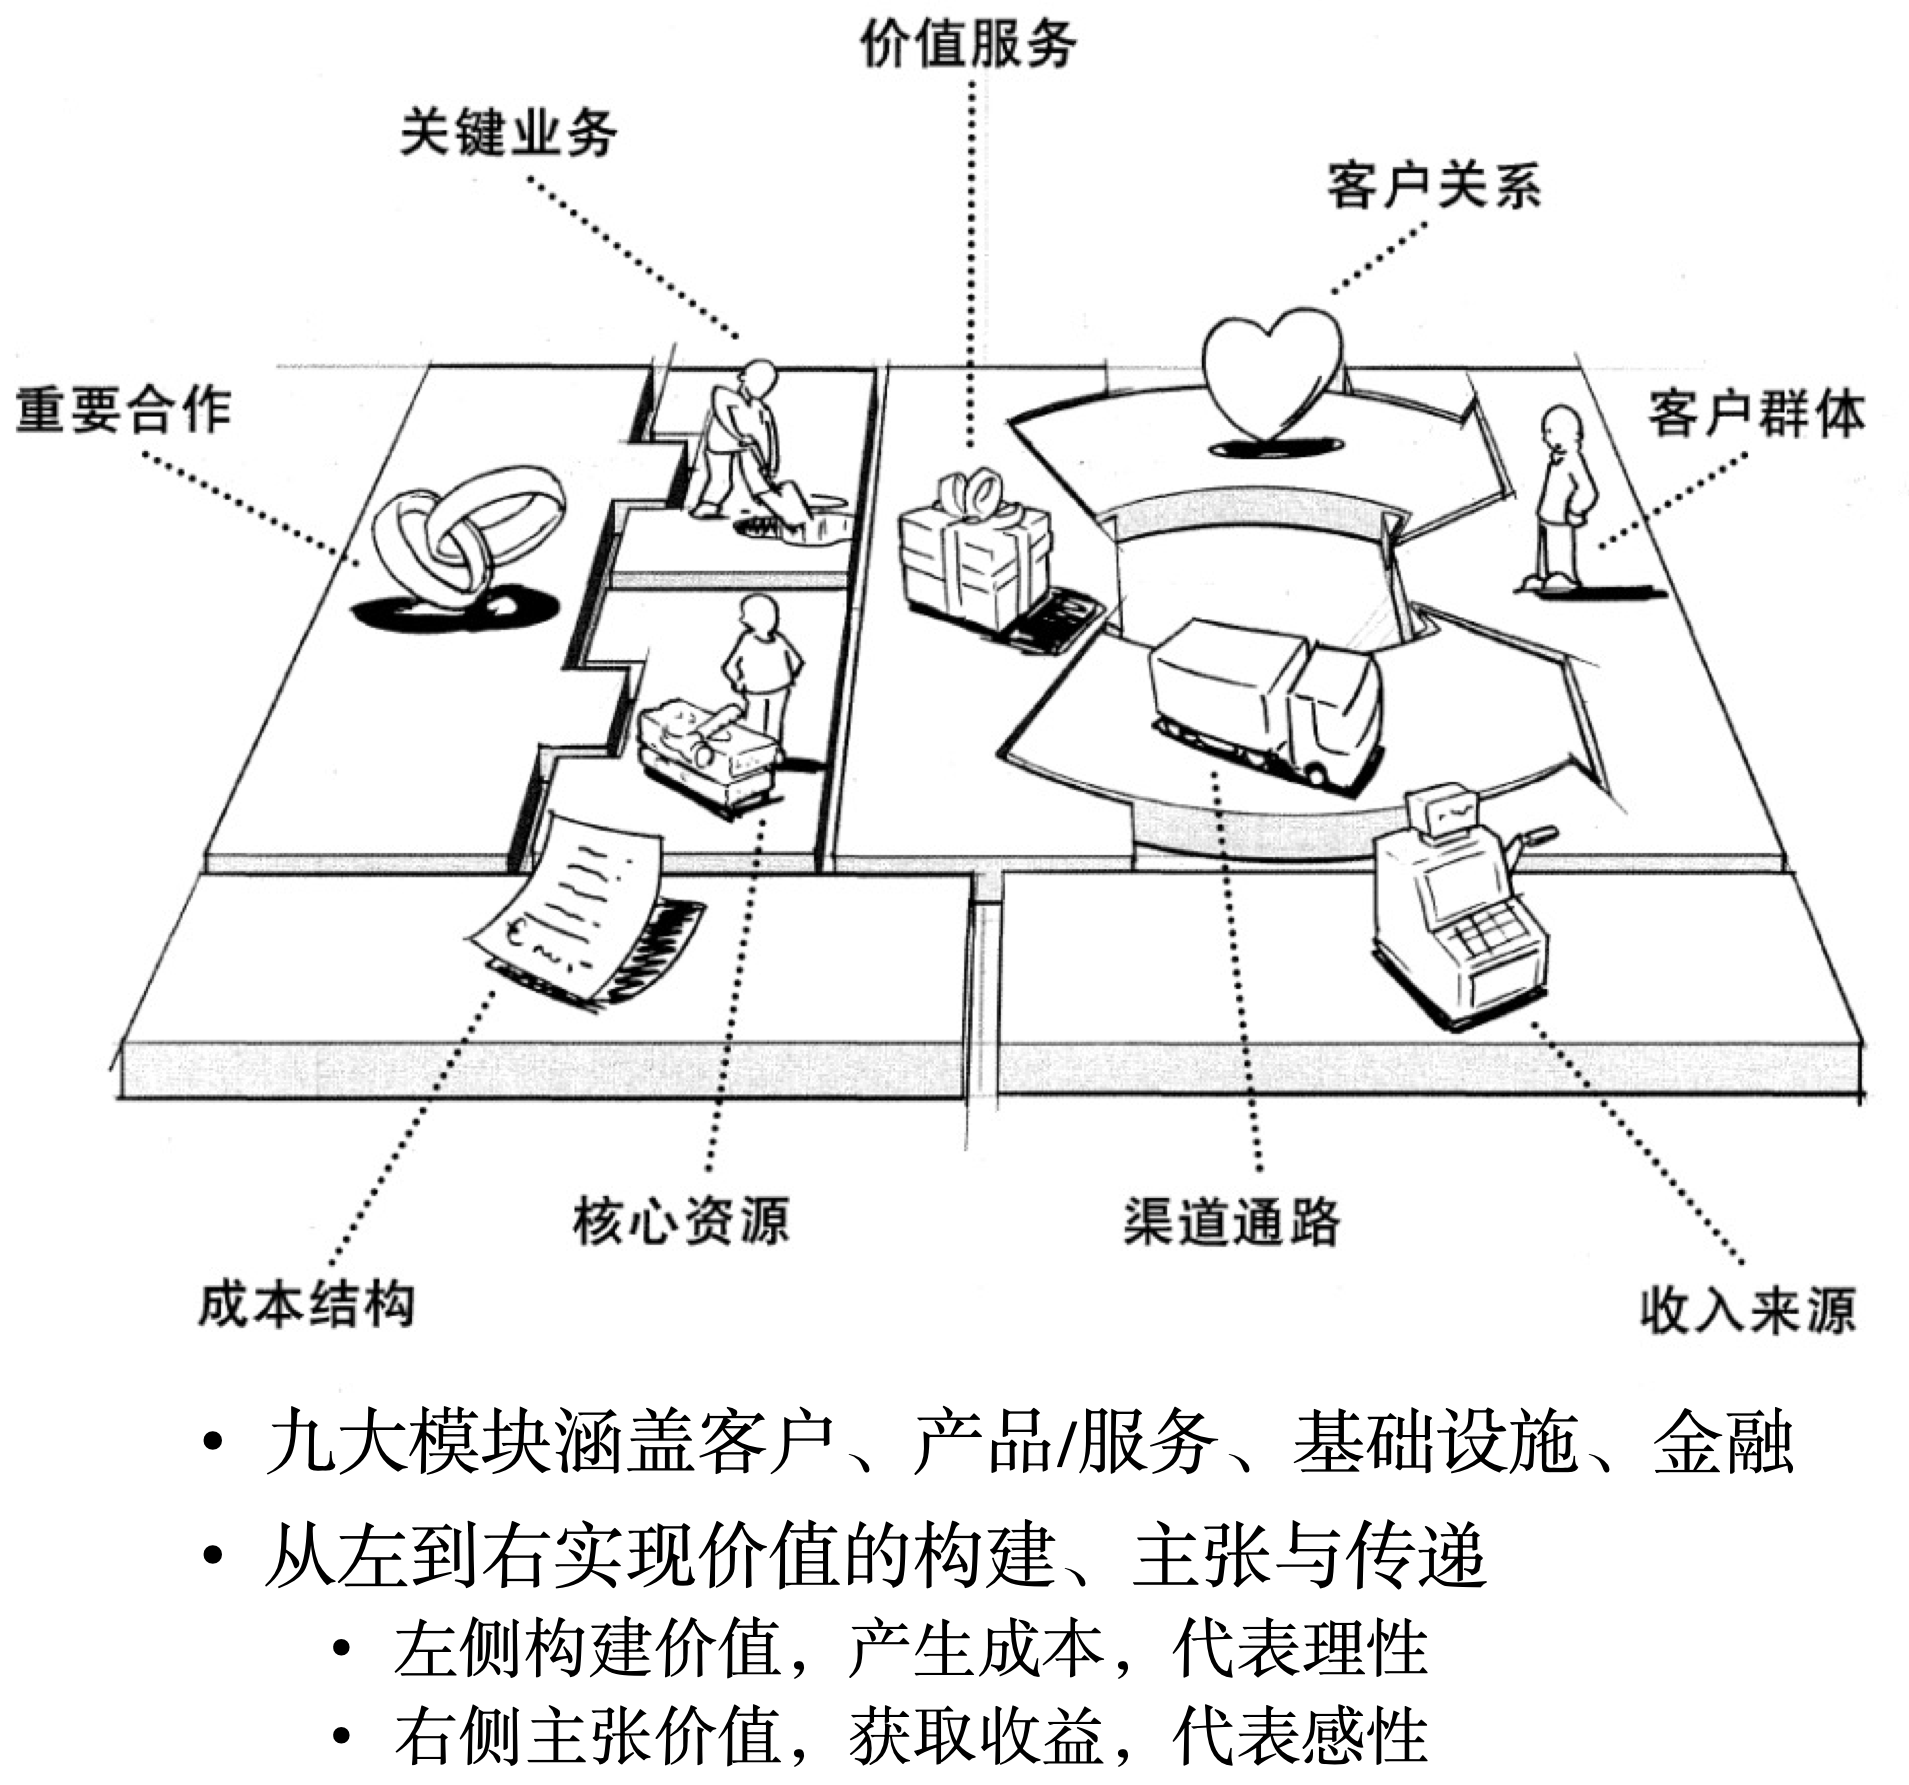
\includegraphics[width=0.58\textwidth]{img/商业模式画布.png}
		\vspace{-0.5em}
	\end{figure}
	
	\subsection{商业模式的九大模块}
	\begin{figure}[H]
		\vspace{-0.5em}
		\centering
		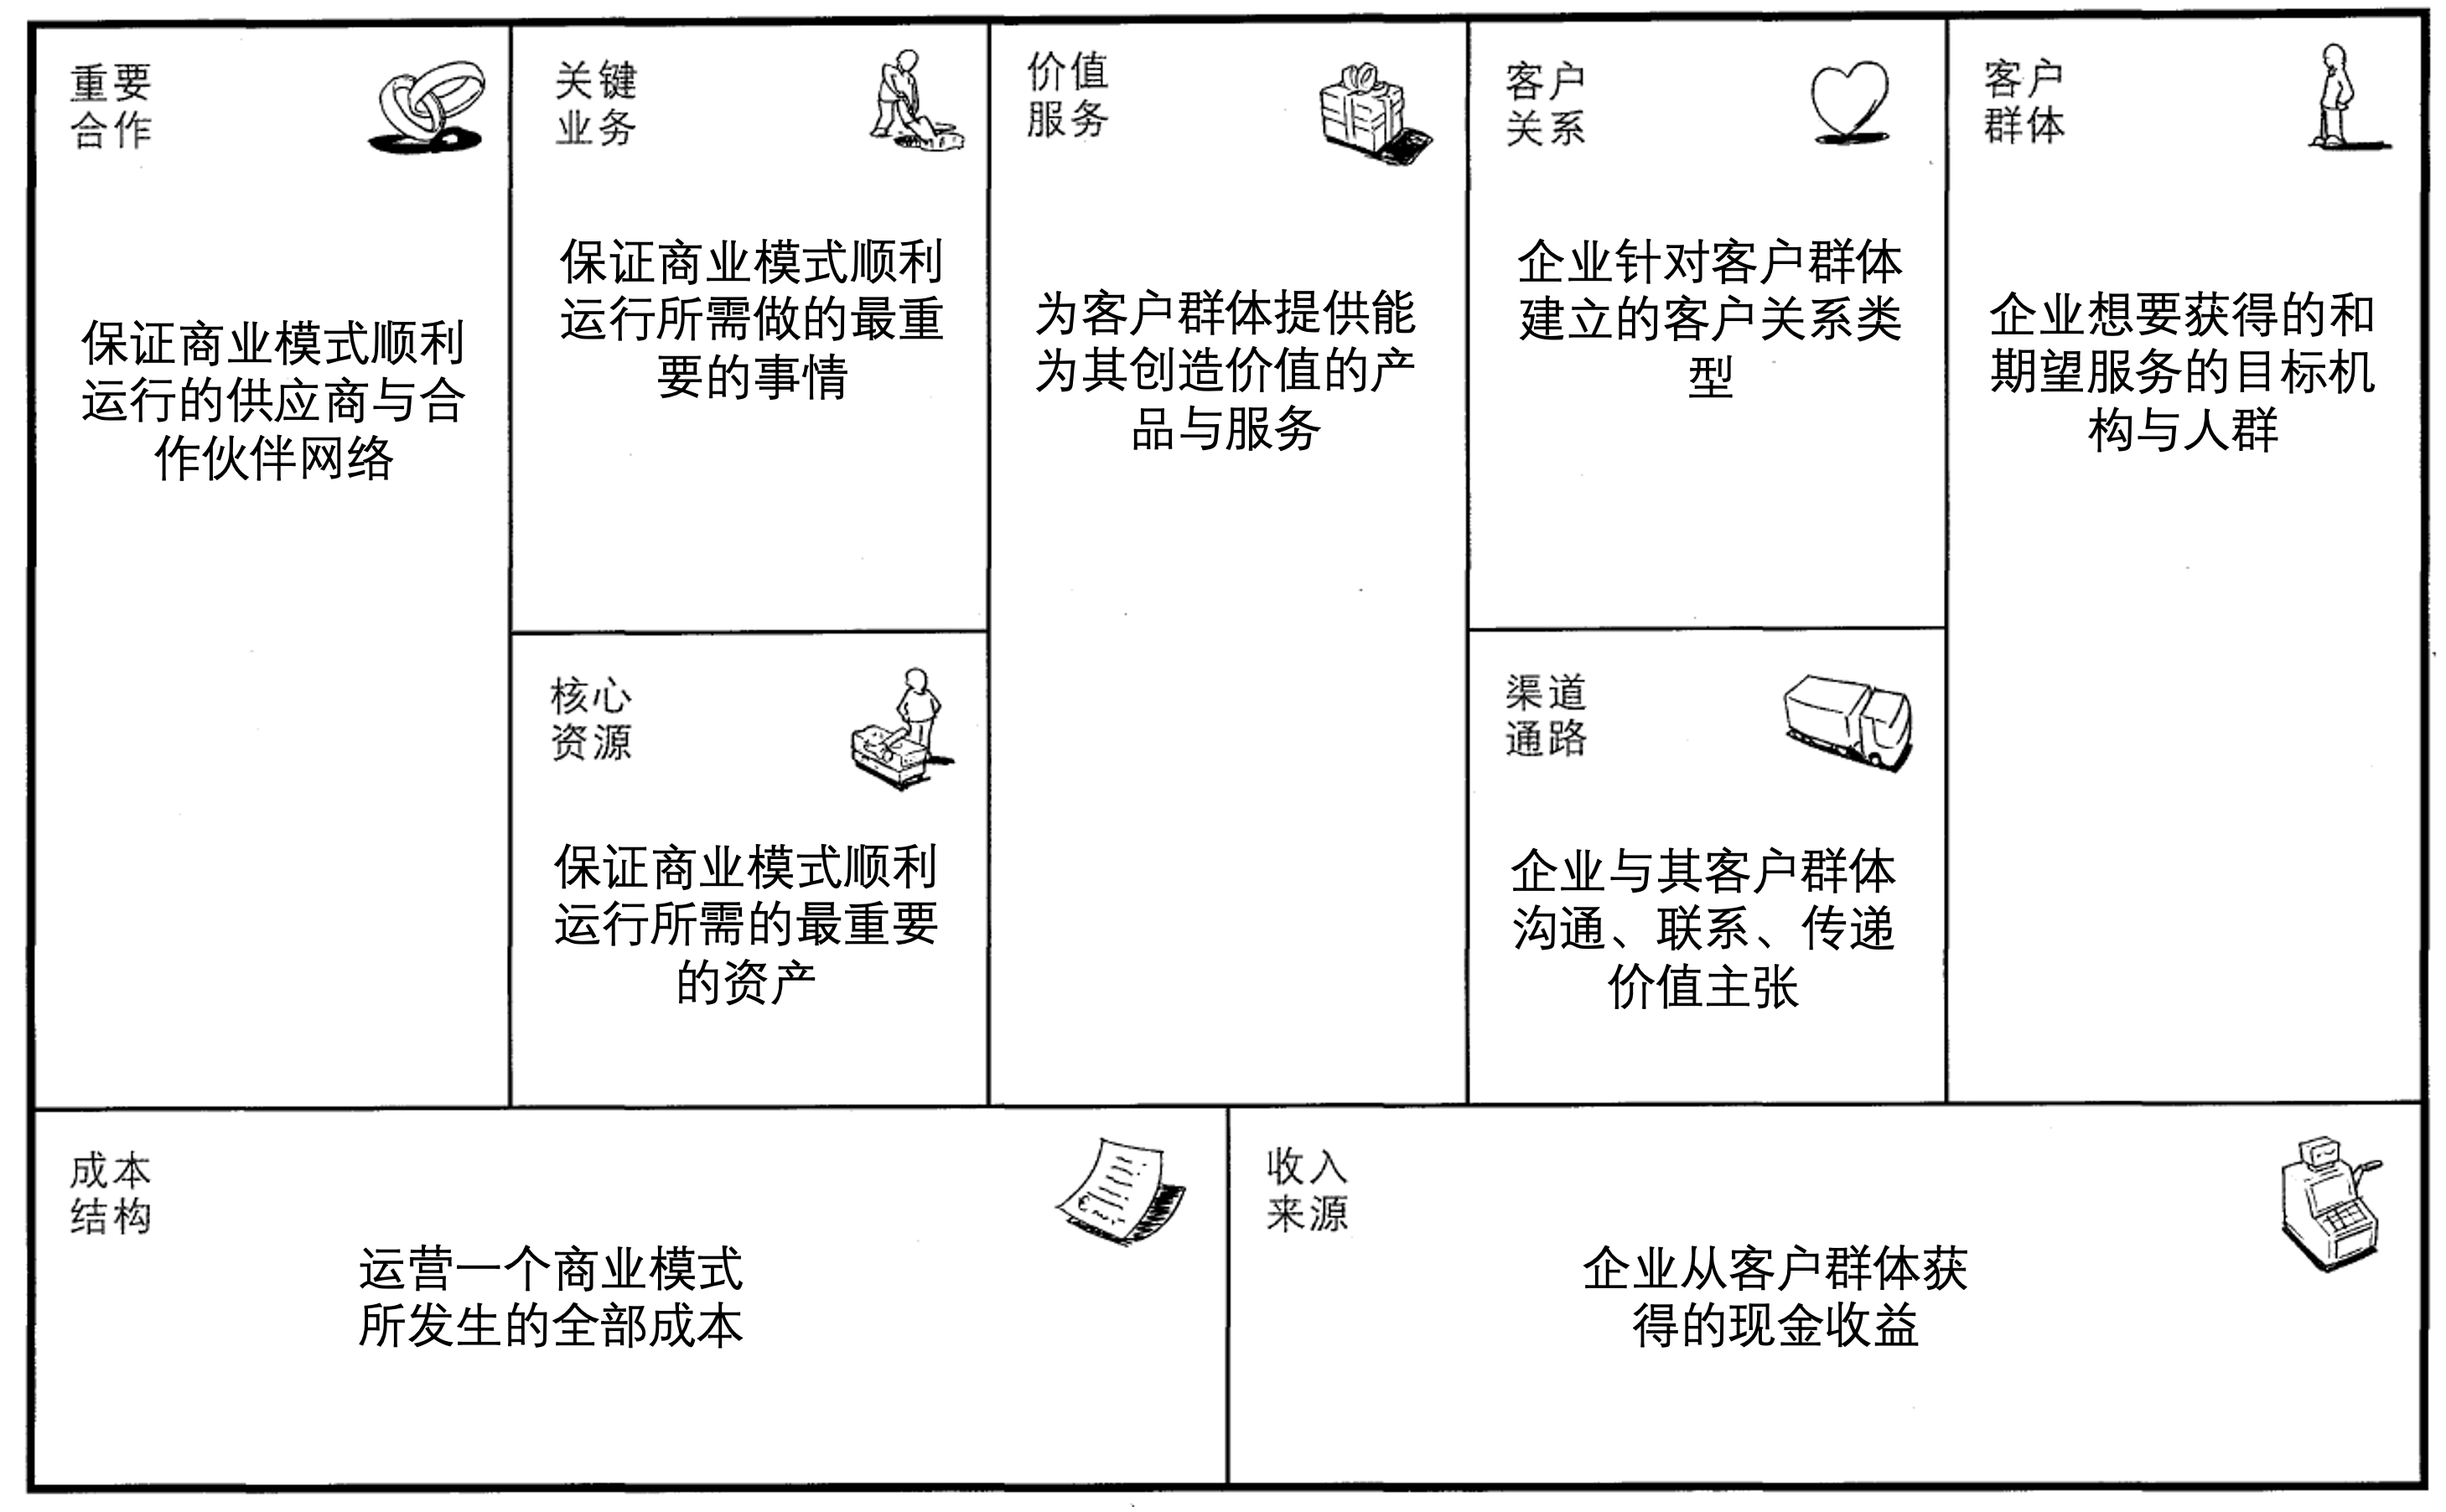
\includegraphics[width=0.72\textwidth]{img/商业模式的九大模块.png}
		\vspace{-0.5em}
	\end{figure}

	\subsubsection{客户细分}
	客户细分(customer segments)描述了一家企业想要获得的和期望服务的不同的目标人群和机构。
	\begin{itemize}
		\item 客户是任何一个商业模式的核心,为了更好地满足客户,企业应按照他们的需求、行为及特征的不同,将客户分成不同的群组。
		\item 一个组织需要谨慎地选择服务于哪个客户群体,以及忽略哪一个客户群体。
	\end{itemize}

	细分客户群体的条件:
	\begin{itemize}
		\item 他们的需求催生了一项新的供给
		\item 需要建立一个新的分销渠道
		\item 需要建立一套新的客户关系类型
		\item 他们产生的利润率显著不同
		\item 他们愿意为某方面的特殊改进而买单
	\end{itemize}


	客户群体的划分有不同的方式,例如:
	\begin{itemize}
		\item 大众市场
		\begin{itemize}
			\item 基于大众化市场的商业模式不会区分客户群体。它们的价值主张、分销渠道、客户关系聚焦于一个庞大的、有着广泛的相似需求和问题的客户群。这种商业模式常见于消费电子产业、大型零售商。
		\end{itemize}
		\item 小众市场
		\begin{itemize}
			\item 迎合的是某一个具体的、专门的客户群体。其价值主张、分销渠道和客户关系皆是根据某小众市场的具体需求量身打造的。这样的商业模式常见于供应商-采购商关系中。
		\end{itemize}
		\item 求同存异的客户群体
		\begin{itemize}
			\item 有的商业模式面向的是有些许差别的需求和问题的多个细分市场,它为每一个客户群体都提供稍有区别的价值主张,常见于各类生产线。
		\end{itemize}
		\item 多元化的客户群体
		\begin{itemize}
			\item 一个面向多元化客户的组织服务的是两个需求和问题迥异的客户群体。例如2006年亚马逊决定通过销售其“云计算”服务来使其零售业务多元化:在线存储空间和服务器点播使用。至此,亚马逊开始了一个面向新的客户群体的自我塑造:互联网公司,即提出了一项全新的价值主张。
		\end{itemize}
		\item 多边平台(多边市场)
		\begin{itemize}
			\item 有的组织服务的是两个或多个相互独立的客户群体。比如一家信用卡公司,既需要一个基数庞大的持卡人群体,又需要一个庞大的接受卡片的商家群体。
		\end{itemize}
	\end{itemize}

	\subsubsection{价值主张}
	价值主张(value propositions)描述的是为某一客户群体提供能为其创造价值的产品和服务。
	\begin{itemize}
		\item 价值主张是客户选择一家公司而放弃另一家的原因,它解决了客户的问题或满足其需求。
		\item 每一个价值主张就是一个产品和(或)服务的组合,这一组合迎合了某一客户群体的要求,价值主张是一家公司为客户提供的利益的集合或组合。
		\item 价值主张可以是创新性的,并带来一种新的或革命性的产品或服务,也可以是与既有的产品或服务相似,但增添了新的特点和属性。
	\end{itemize}

	价值主张通过针对某个群体的需求定制一套新的元素组合来为该群体创造价值,所创造的价值可以是数量上的(如价格、服务响应速度等),也可以是质量上的(如设计、客户体验)。
		
	对有益于容户价值创造的因素:
	\begin{itemize}
		\item 创新
		\begin{itemize}
			\item 有的价值主张满足的是客户之前未曾察觉的全新的需求,因为之前并没有类似的产品或服务存在。这一类经常,但并非总是与科技相关。比如手机,在移动通信中创造了一个新的产业。
		\end{itemize}
		\item 性能 
		\begin{itemize}
			\item 改进产品或服务的性能是一项传统而普遍的创造价值的方式。个人计算机产业一直以来便采用这种方式,即不断向市场提供性能更加强大的计算机。但增进性能是有局限性的。
		\end{itemize}
		\item 定制
		\begin{itemize}
			\item 针对某些客户或客户群体的某项需求提供定制的产品或服务能够创造价值。大规模定制和客户参与创造的生产方式凸显了其重要性。这种方式在提供了定制化的产品或服务的同时,保持了生产规模化的经济性。
		\end{itemize}
		\item 保姆式服务
		\begin{itemize}
			\item 帮用户完成任务并创造价值,例如劳斯莱斯提供的飞机引擎维护服务。           
		\end{itemize}
		\item 设计
		\begin{itemize}
			\item 设计是一个重要但很难量化的元素。一个产品可能由于其出色的设计而鹤立鸡群。在时尚产业和消费电子产业,设计对于价值主张而言尤其重要。
		\end{itemize}
		\item 品牌/地位
		\begin{itemize}
			\item 客户可以简单地通过使用和展示某一品牌而获得价值。例如,佩戴一块劳力士手表,彰显了财富。           
		\end{itemize}
		\item 价格
		\begin{itemize}
			\item 以更低的价格提供相同的价值是满足价格敏感型客户群体的需求的普遍方式。但低价格主张对于商业模式的其他模块都有着重要的影响例如,廉价航空专门设计了一整套商业模式来实现低成本飞行。
		\end{itemize}
		\item 缩减成本
		\begin{itemize}
			\item 帮助客户节约成本是创造价值的重要方式。例如服务外包产业。
		\end{itemize}
		\item 风险控制
		\begin{itemize}
			\item 为客户购买的产品或服务降低风险,能够为其创造价值。对于一个二手车买家而言,一年内保修的政策为买家降低了购车后的故障和维修风险。
		\end{itemize}
		\item 可获得性
		\begin{itemize}
			\item 帮助客户获得之前他们无法获得的产品和服务也是创造价值的方式。这一方式可能得益于商业模式的创新、科技的创新,或两种创新共同作用的结果。例如,奈特捷公司使得合伙购买私人飞机这种方式流行起来。
		\end{itemize}
		\item 便利性/实用性
		\begin{itemize}
			\item 让产品使用起来更方便或操作起来更简单也可以创造相当大的价值。通过iPod和iTunes,苹果公司为客户提供了数字音乐从搜索、购买,到下载和使用一整套前所未有的便捷体验。苹果也因此主导了整个数字音乐市场。
		\end{itemize}
	\end{itemize}
		
		
	\begin{itemize}
		\item 让事情更简单(痛点):价格、缩减成本、便利性/实用性
		\item 让事情更“复杂”(收益):定制、设计、品牌地位、可获得性
		\item 让事情更“透明”(痛点):风险控制、一站式服务
	\end{itemize}

	\subsubsection{渠道通路}
	渠道通路(channels)描述的是一家企业如何同它的客户群体达成沟通并建立联系,以向对方传递自身的价值主张。
	\begin{itemize}
		\item 与客户的交流、分销和销售渠道构成了一个企业的客户交互体系。
		\item 渠道通路在客户体验中扮演着重要角色的客户触点。
		\item 是商业真正的秘密,与产品设计的关系微妙(重合度小,却又容易受到产品口碑风险的冲击),容易积累收益但波动性极大、风险高。
	\end{itemize}

	渠道通路的作用包括以下几点:
	\begin{itemize}
		\item 使客户更加了解公司的产品和服务;
		\item 帮助客户评估一家公司的价值主张;
		\item 使得客户得以购买某项产品和服务;
		\item 向客户传递价值主张;
		\item 向客户提供售后支持。
	\end{itemize}


	一个组织可以选择使用自有渠道来与它的客户建立联系,也可以选择合作方的渠道,或者两者兼用。
	\begin{itemize}
		\item 自有渠道可以是直接的,比如内部销售团队或者网站;也可以是间接的,如该组织名下的或负责运营的零售商店
		\item 合作方渠道是间接的,并且范围很广,比如批发分销渠道、销售渠道或者合作方运营的网站
		\item 使用合作方渠道导致利润更低,但这些渠道可以帮助一个组织扩张客户的范围,并且从合作方的强项中获益
		\item 自有渠道尤其是直接的自有渠道利润较高,但渠道本身的建立和运营成本也会很高
		\item 难点在于整合各种类型的渠道,并找到最佳平衡,以创造最佳的客户体验和最大化的收益
	\end{itemize}
	
	\begin{figure}[H]
		\vspace{-0.5em}
		\centering
		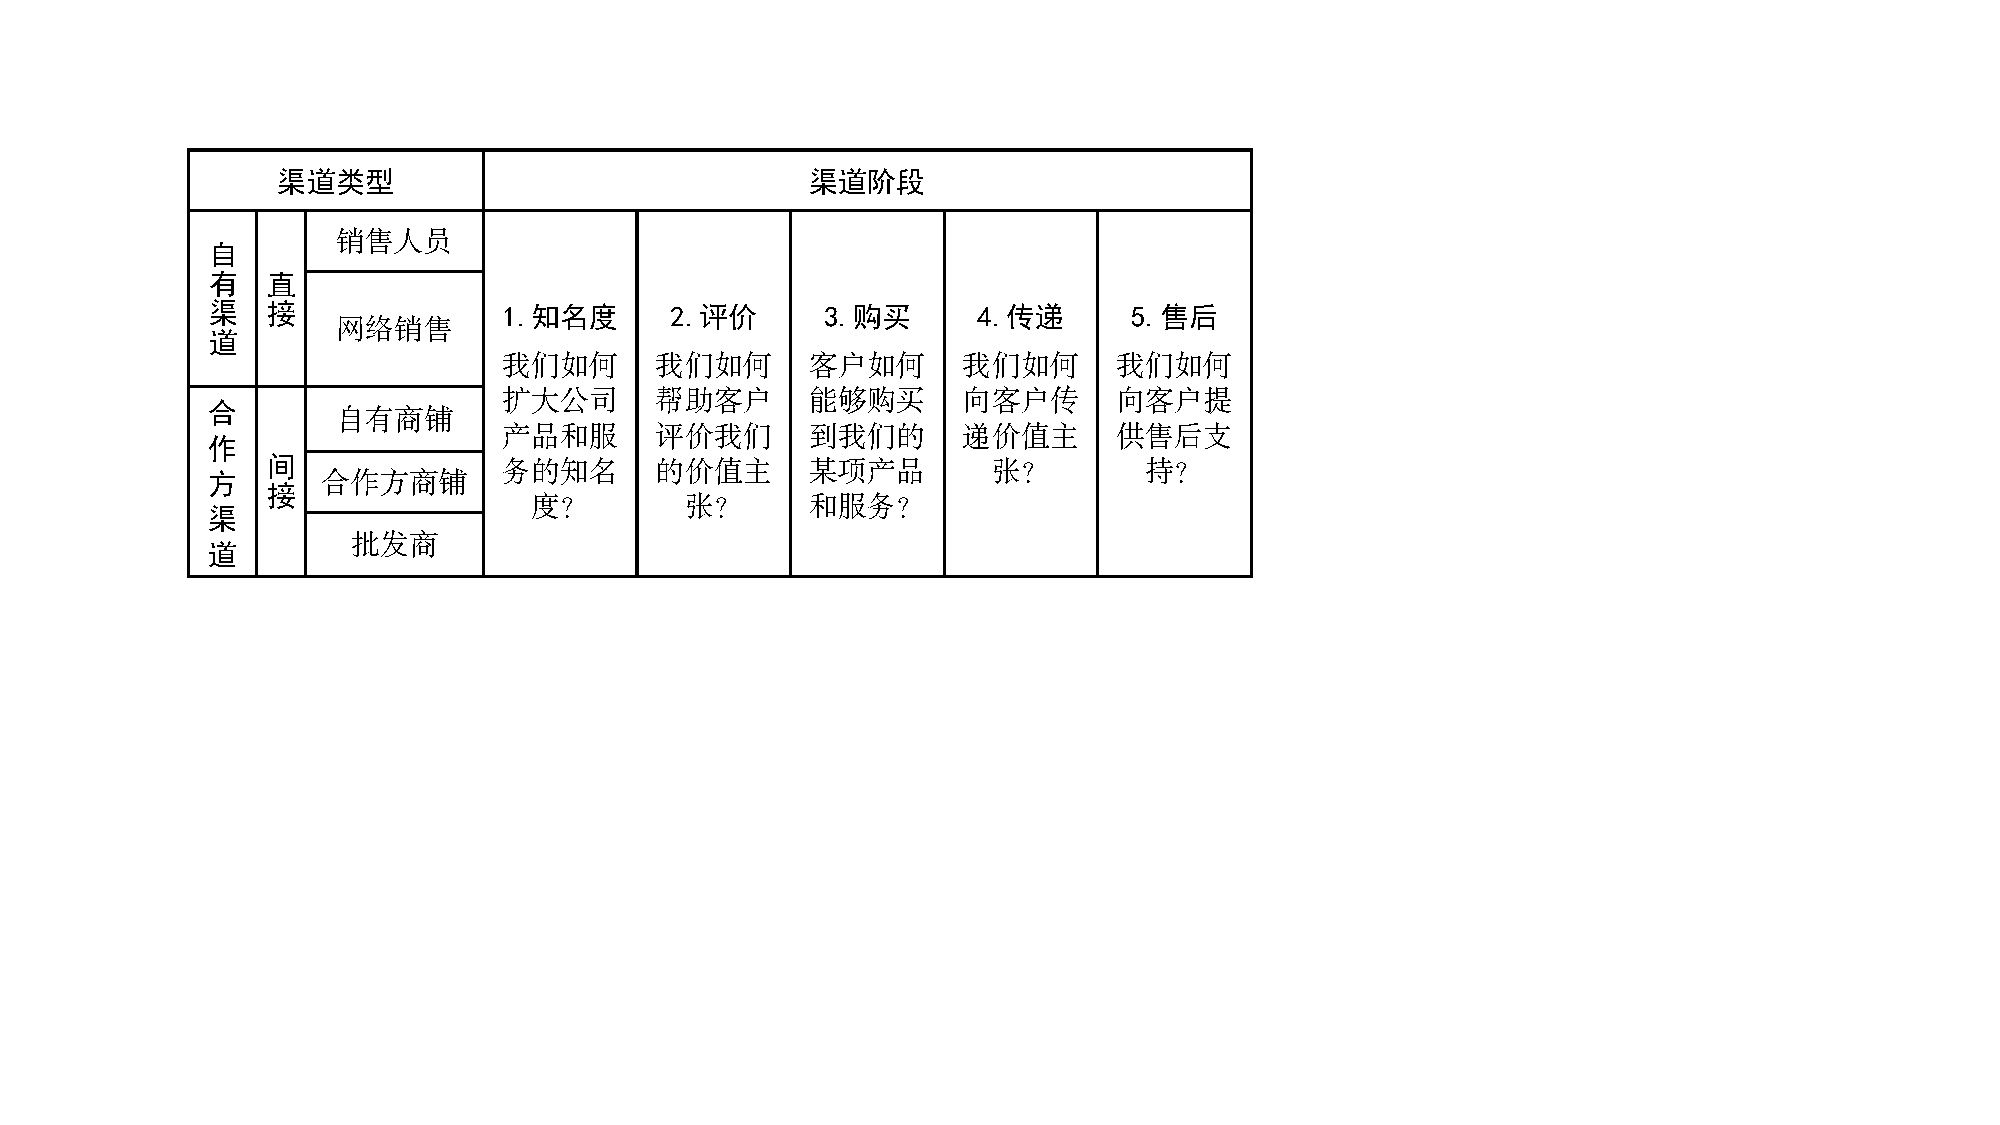
\includegraphics[width=0.7\textwidth]{img/渠道通路的类型和阶段.pdf}
		\vspace{-0.5em}
	\end{figure}

	\subsubsection{客户关系}
	客户关系(customer relationships)描述的是一家企业针对某一个客户群体所建立的客户关系的类型。
	\begin{itemize}
		\item 企业需要明确对每一个客户群体欲建立何种关系类型。
		\item 客户关系可能是由以下动机驱动的:
		\begin{itemize}
			\item 开发新的客户
			\item 留住原有客户
			\item 增加销售量(或单价)
		\end{itemize}
	\end{itemize}

	客户关系的类型:
	\begin{table}[H]
		\centering
		\begin{tabularx}{0.8\textwidth}{|l|X|}
		\hline
		客户关系       & \multicolumn{1}{c|}{具体描述}                                                                                                   \\ \hline
		私人服务       & 这种客户关系是基于人际互动的。客户可以与客户代表进行交流并在销售过程中以及购买完成之后获得相应的帮助。这种互动可以发生在购买的现场,通过呼叫中心、电邮或其他渠道进行。                                         \\ \hline
		专属私人服务     & 这种客户关系要求为每一个客户指定一个固定的客户经理。这是一种最深层的最私人的客户关系类型,通常需要很长时间的积累。例如,私人银行服务,为高净值客户指定专门的银行经理。类似的客户关系可以在其他行业中找到,比如大容户经理负责维系与重要客户的私人关系。 \\ \hline
		自助服务       & 在这种客户关系中,企业无须直接维护与客户的关系。企业只需为客户提供一切自助服务所需要的渠道。                                                                              \\ \hline
		自动化服务      & 此类型的客户关系将相对复杂的客户自助服务形式与自动化流程相结合。例如,个人在线资料使得客户可以获得定制化的服务。自动化服务可以识别客户身份及其特点,并符合预订单和交易内容的信息。最好的自动化服务可以模仿人际关系交往(比如推荐书或电影)。      \\ \hline
		社区         & 企业使用用户社区来融入客户以预判市场未来发展的方向,管理客户预期,例如花粉俱乐部、小米之家等。                                                                             \\ \hline
		与客户协作,共同创造 & 更多的企业开始超越传统的买卖关系,与客户合作共同创造价值。亚马迅邀请其客户撰写书评,如此就为其他书友创造了价值。有的企业吸引用户来帮助他们共同设计有创造性的新产品。                                          \\ \hline
		\end{tabularx}
		\end{table}

	\subsubsection{收入来源}
	收入来源(revenue streams)代表企业从每一个客户群体获得的现金收益(须从收益中扣除成本得到利润)。
	\begin{itemize}
		\item 每一个收益来源中可能包含不同的价格机制,比如固定目录价、议价、竞价、根据市场浮动的价格、根据购买数量浮动的价格,以及收益管理系统(定价)
		\item 一个商业模式可能包含的收益来源分为以下两种不同的类型:
		\begin{itemize}
			\item 交易收入由客户一次性支付产生
			\item 持续收入:因向客户传递了新的价值主张或提供了售后支持而带来的客户持续支付
		\end{itemize}
	\end{itemize}

	创造收入来源的方式有很多种:
	\begin{itemize}
		\item 资产销售
		\begin{itemize}
			\item 最普遍被认知的收入来源就是实物产品所有权的出售。例如亚马逊通过网站销售图书、音乐、消费类电子产品等商品。
		\end{itemize}
		\item 使用费
		\begin{itemize}
			\item 这一收入来源是因对某种具体服务的使用而产生的。对该服务使用得越多,消费者支付的就越多。例如电信运营商根据用户使用电话的分钟数收费。
		\end{itemize}
		\item 会员费
		\begin{itemize}
			\item 这种收入来源通过向用户销售某项服务持续的使用权限实现。例如健身房向用户销售月卡或年卡以限定会员对健身器材的使用时限。
		\end{itemize}
		\item 租赁
		\begin{itemize}
			\item 这种收入来源产生于:将某一特定资产在某一个时期专门供给某人使用并收取一定费用。对出租者而言,这种做法提供的是经常性收入。同时对于租赁者而言,仅需要承担一个限定时间内的费用而无须承担整个所有权所耗费的成本。
		\end{itemize}
		\item 许可使用费
		\begin{itemize}
			\item 这种收入来源来自:向用户授予某种受保护知识产权的使用权,并向其收取许可使用费。许可使用费使得资源持有者无须生产产品或进行任何商业化操作,而仅凭其对资源的所有权获取收益。许可使用费在传媒行业十分常见,内容所有人会持有版权,但是将使用权提供给第三方。相似地,在科技产业中,专利持有者将专利使用权提供给其他公司使用并收取专利使用费。
		\end{itemize}
		\item 经纪人佣金
		\begin{itemize}
			\item 这一收入来源于向双方或多方提供的中介服务。例如,信用卡发卡机构针对每一笔交易向商家和持卡人按交易额度的一定百分比收取费用。
		\end{itemize}
		\item 广告费
		\begin{itemize}
			\item 这种收入来源来自为某种产品、服务或品牌做广告的费用。传统的传媒业和活动策划的收入很大程度上依赖于广告上的收人。近此年其他产业,包括软件业和服务业,也开始更多地依赖于广告收入。
		\end{itemize}
	\end{itemize}

	定价机制:
	\begin{table}[H]
		\centering
		\resizebox{\textwidth}{!}{
		\begin{tabular}{|c|l|c|l|}
		\hline
		\multicolumn{2}{|c|}{\begin{tabular}[c]{@{}c@{}}\textbf{固定价格}\\ 基于静态变量预定的价格\end{tabular}} & \multicolumn{2}{c|}{\begin{tabular}[c]{@{}c@{}}\textbf{浮动价格}\\ 价格依据市场条件变化\end{tabular}}             \\ \hline
		目录价        & \begin{tabular}[c]{@{}l@{}}对个别产品、服务或其他价值主\\ 张设定的固定价格\end{tabular}   & 谈判(议价) & \begin{tabular}[c]{@{}l@{}}双方或多方的价格谈判,取决于谈判\\ 各方的谈判能力和技巧\end{tabular}             \\ \hline
		基于产品特性的    & \begin{tabular}[c]{@{}l@{}}基于某项价值主张的数量或质量的\\ 定价\end{tabular}        & 收益管理   & \begin{tabular}[c]{@{}l@{}}价格基于库存及发生购买的时间\\ (通常用于易耗资源,如宾馆房间和\\ 航班机位)\end{tabular} \\ \hline
		基于客户群的     & \begin{tabular}[c]{@{}l@{}}基于某一客户群体的类型和特征\\ 的定价\end{tabular}        & 实时市场价格 & 价格根据需求变化动态变动                                                                      \\ \hline
		基于数量的      & 基于购买数量的定价                                                           & 拍卖     & 根据竞价的结果决定                                                                         \\ \hline
		\end{tabular}
		}
		\end{table}

	\subsubsection{核心资源}
	核心资源(key resources)描述的是保证一个商业模式顺利运行所需的最重要的资产。
	\begin{itemize}
		\item 每一种商业模式都需要一些核心资源。这些资源使得企业得以创造并提供价值主张,获得市场,保持与某个客户群体的客户关系并获得收益。
		\item 核心资源可包括实物资源、金融资源、知识性资源以及人力资源。核心资源可以是自有的,也可以通过租赁获得,或者从重要合作伙伴处获得。
	\end{itemize}

	核心资源可以分为如下几类:
	\begin{itemize}
		\item 实物资源
		\begin{itemize}
			\item 这一范畴包括实物资产,如生产设备、房屋、车辆、机器、系统、销售点管理系统及分销渠道。作为零售商,沃尔玛和亚马逊都非常依赖实物资源,这些资源通常都是资本密集型的。沃尔玛在全球范围内拥有庞大的仓储网络以及配套的物流设备。亚马逊拥有一套庞大的IT、仓储及物流基础设施。
		\end{itemize}
		\item 知识性资源
		\begin{itemize}
			\item 知识性资源如品牌、专营权、专利权、版权、合作关系以及客户数据库在一个强大的商业模式中扮演着越来越重要的角色。
		\end{itemize}
		\item 人力资源
		\begin{itemize}
			\item 每一家企业都需要人力资源,但人力资源对于某些商业模式而言却是尤其重要的。例如,在知识密集型产业和创新产业中,人力资源就是最关键的。
		\end{itemize}
		\item 金融资源
		\begin{itemize}
			\item 有些商业模式依赖金融资源或金融保障,比如现金、信用额度或者用于吸引关键雇员的股票期权池。例如,电信运营商爱立信在自己的商业模式中加入了金融杠杆。爱立信可以选择向银行或资本市场融资,然后将收益的一部分为购买设备的客户提供卖方融资,这就更好地保证了订单落入爱立信而非竞争对手手中。
		\end{itemize}
	\end{itemize}


	\subsubsection{关键业务}
	关键业务(key activities)描述的是保障其商业模式正常运行所需要做的最重要的事情。
	\begin{itemize}
		\item 每一个商业模式都有着一系列的关键业务,这些业务是一个企业成功运营所必须采取的最重要的行动。
		\item 同核心资源一样,它们是企业为创造和提供值主张、获得市场、维系客户关系以及获得收益所必需的,关键业务也因不同的商业模式类型而异。
		\item 对于软件商微软而言,关键业务就是软件开发;对于个人电脑生产商戴尔而言,关键业务则包含了供应链管理;对于咨询公司麦肯锡而言,关键业务包括了解决方案的提供。
	\end{itemize}

	关键业务可以分为如下几类:
	\begin{itemize}
		\item 生产
		\begin{itemize}
			\item 这些活动涉及以较大的数量或上乘的质量,设计、制造以及分销产品。生产活动在制造企业的商业模式中占支配地位。
		\end{itemize}
		\item 解决方案
		\begin{itemize}
			\item 这个类型的关键活动涉及为个体客户的问题提供新的解决方案。咨询公司、医院及其他服务性机构的运营,就是典型地受解决问题相关的活动支配的例子。这类商业模式需要的活动包括知识管理以及持续的培训等。
		\end{itemize}
		\item 平台/网络
		\begin{itemize}
			\item 在将平台作为关键资源的商业模式中,与平台以及网络相关的关键活动占据着支配地位。网络、配对平台、软件甚至品牌都可以发挥平台的作用。Visa公司为Visa$^\circledR$信用卡的商家、持卡人及银行之间搭建的交易平台,该公司的商业模式要求公司的关键活动与该平台相关。微软的商业模式要求其对其他商家的软件和Windows$^\circledR$操作系统的交互界面进行管理。这个类型的关键活动涉及了平台管理、新服务的启动以及平台的升级。
		\end{itemize}
	\end{itemize}


	\subsubsection{重要合作}
	重要合作(key partnerships)描述的是保证一个商业模式顺利运行所需的供应商和合作伙伴网络。

	可以将重要合作分为以下四种不同的类型:
	\begin{enumerate}[label=\arabic*.]
		\item 非竞争者之间的战略联盟
		\item 合作:竞争者之间的战略合作
		\item 为新业务建立合资公司
		\item 为保证可靠的供应而建立的供应商和采购商关系
	\end{enumerate}

	建立合作伙伴关系的三种动机:
	\begin{itemize}
		\item 优化及规模效应
		\begin{itemize}
			\item 最基本的一种合作关系或者买卖关系的类型就是以优化资源以及活动的配置为目的的。要一家公司拥有全部所需的资源并亲自完成所有的生产、服务环节并不合理。此类合作关系的建立通常是为了降低成本,主要采取外包或基础设施共享的形式。
		\end{itemize}
		\item 降低风险和不确定性
		\begin{itemize}
			\item 竞争环境以不确定性为特征,合作关系的建立可以帮助企业在竞争环境中降低风险。互为竞争对手的企业在某一个领域建立战略联盟,而在其他领域保持竞争关系的做法是很常见的。例如,蓝光技术是由一组全球领先的消费电子、个人电脑及内容提供商联合开发的光盘格式。各商家一方面联手向市场推出蓝光技术,另一方面又在蓝光产品的销售领域相互竞争。
		\end{itemize}
		\item 特殊资源及活动的获得
		\begin{itemize}
			\item 很少有公司拥有其商业模式下所需要的全部资源或者选择亲自完成所有的生产服务活动。更多的情况下,它们通过依赖其他占有某项资源或专注于某种生产活动的公司来实现其能力的拓展。这种类型的合作关系的动机在于获得知识、获得某种资质或者接近某个客户群体。例如,一个移动电话生产商,会选择为它们的手机搭载一个操作系统,而不会选择自主研发。
		\end{itemize}
	\end{itemize}

	\subsubsection{成本结构}
	成本结构(cost structure)描述的是运营一个商业模式所发生的全部成本。
	\begin{itemize}
		\item 创造和传递价值,维护客户关系,以及创造收益都会发生成本
		\item 在确定了核心资源、关键业务以及重要合作的情况下,成本核算就会变得相对容易
		\item 也有以低成本结构为核心的商业模式
	\end{itemize}

	商业模式的成本结构可以宽泛地分为两个等级
	\begin{itemize}
		\item 成本导向:聚焦于最大限度将成本最小化,目标在于创造并维持极尽极简的成本结构
		\item 价值导向:有些企业在商业模式设计中,更少关注成本,而更多地关注价值创造。通常更高端的价值主张以及高度的个性化服务是价值导向商业模式的特点。
	\end{itemize}

	成本结构有以下特点:
	\begin{itemize}
		\item 固定成本
		\begin{itemize}
			\item 不因产品及服务的产量而改变的成本,包括员工工资、租金、生产设备有的商业项目,比如生产型企业,以高比例的固定成本为特点。
		\end{itemize}
		\item 可变成本
		\begin{itemize}
			\item 随着产品及服务的产量而同比例变化的成本。有的商业项目,比如音乐节,以高比例的可变成本为特征。
		\end{itemize}
		\item 规模经济
		\begin{itemize}
			\item 企业的产出扩大,会带来成本优势例如,大型企业享有大宗商品采购价。诸如此类的因素导致随着总产出的增加,平均单位成本的降低。
		\end{itemize}
		\item 范围经济
		\begin{itemize}
			\item 企业的经营范围扩大,会带来成本优势。例如,在大型企业中,同一个营销活动或分销渠道上可以供多个产品使用。
		\end{itemize}
	\end{itemize}

	\subsection{苹果公司iPod/iTunes商业模式}
	\begin{figure}[H]
		\centering
		\vspace{-0.5em}
		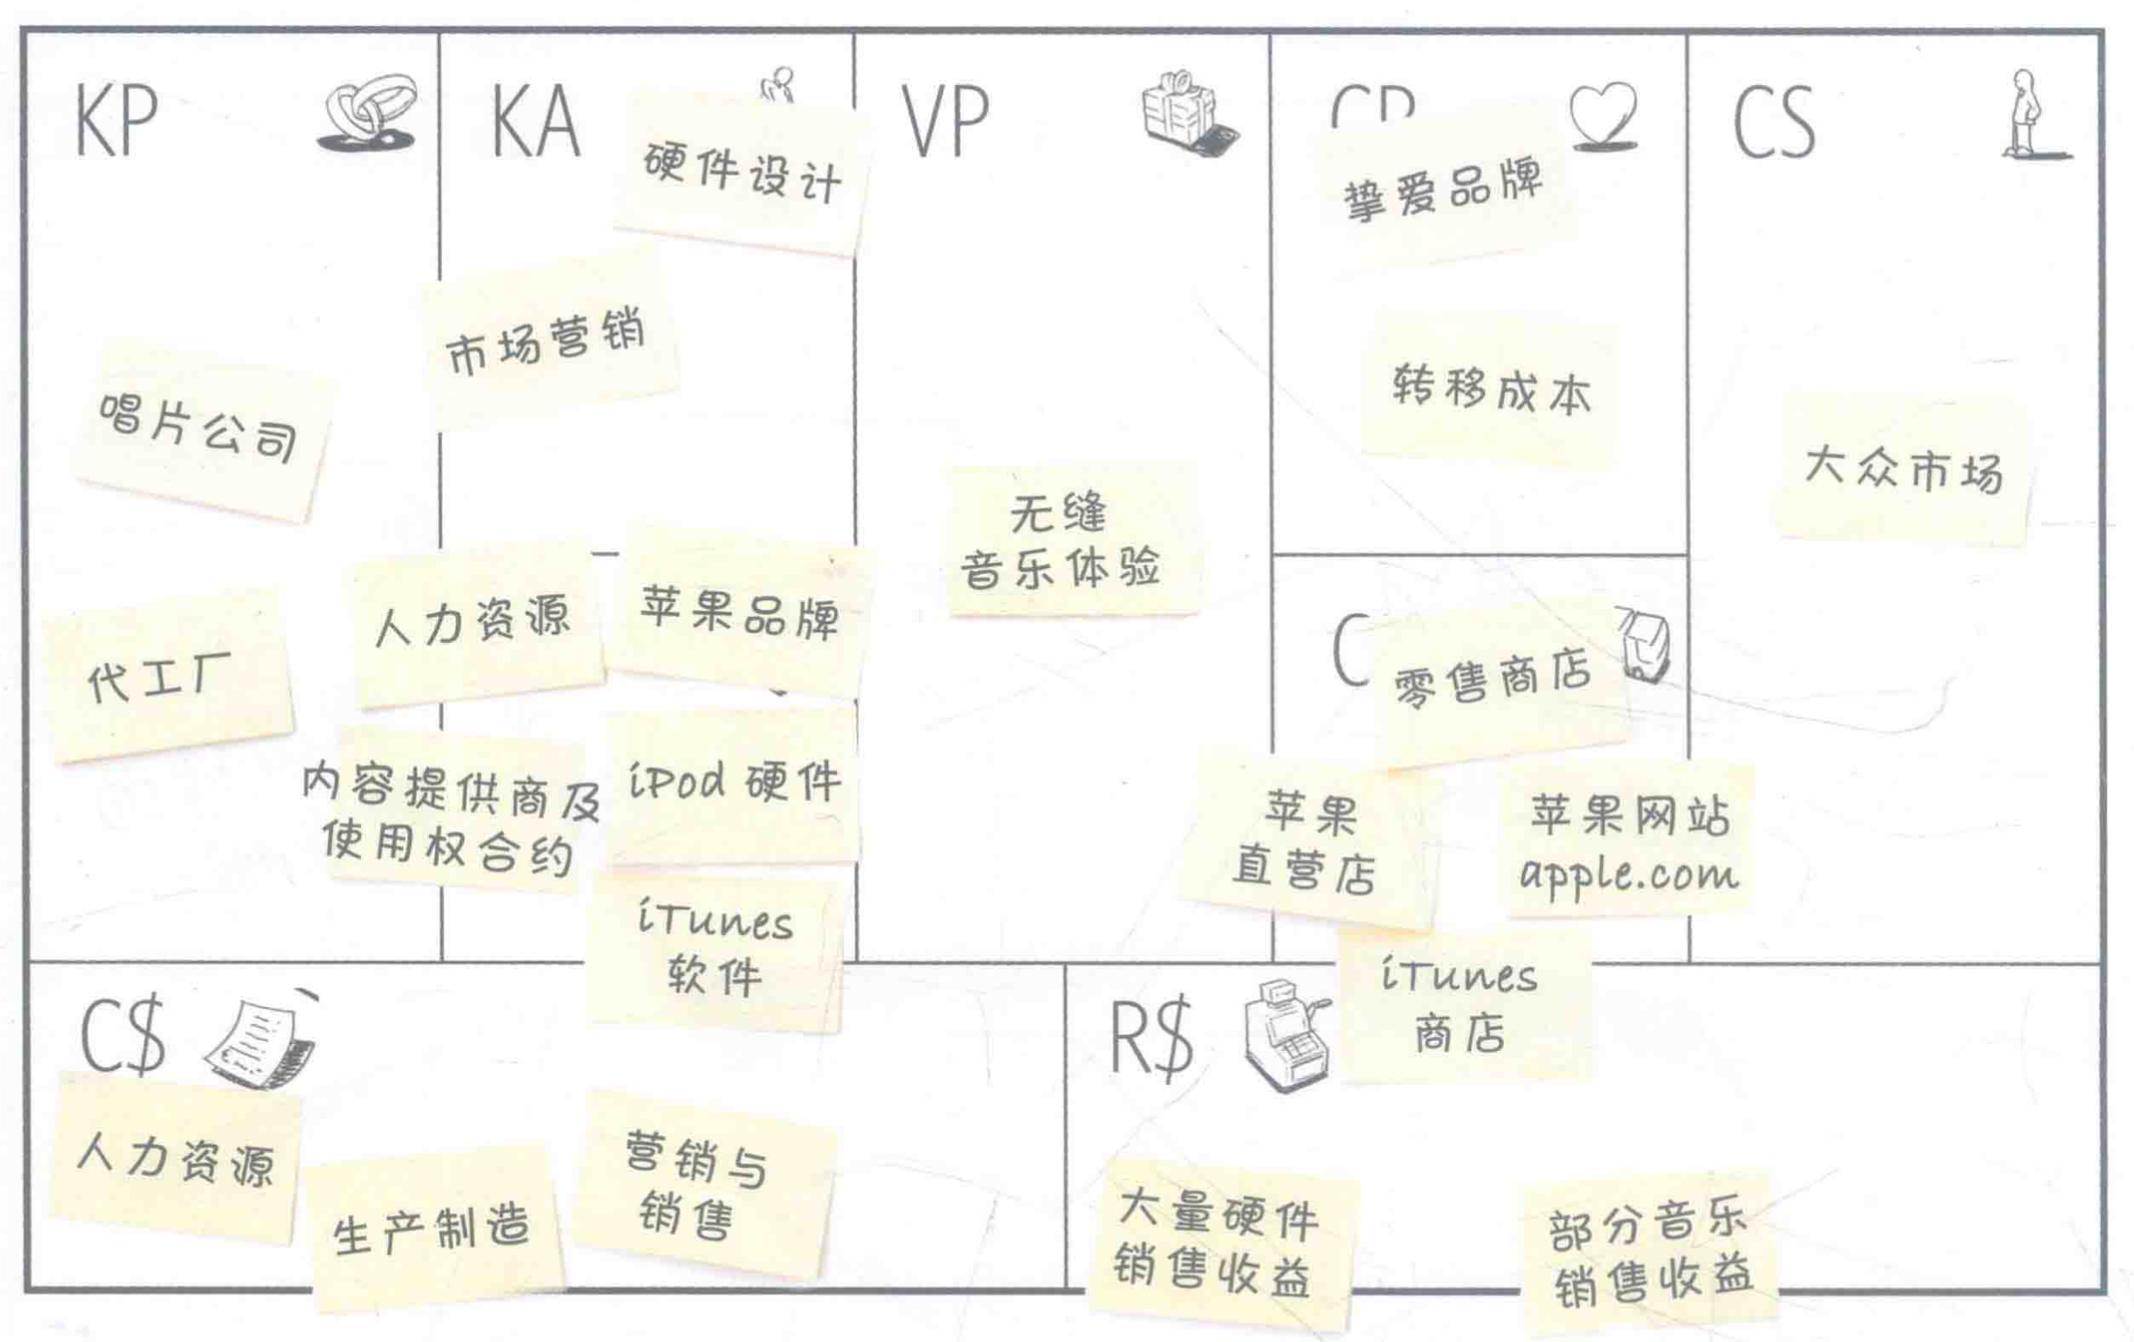
\includegraphics[width=0.8\textwidth]{img/iPod:iTunes商业模式.png}
		\vspace{-0.5em}
	\end{figure}

	\subsection{商业模式画布的使用}
	\begin{itemize}
		\item 帮助找到企业自身定位,具象化公司现有的商业模式以及未来适用的商业模式
		\item 帮助企业策划其自身的转型及退出企业的过程
		\item 帮助艺术家、文化产业生产企业以及游戏设计师设计文化创意产业的创新商业模式
		\item 帮助非营利项目组建过程中的领导团队的设计及编排
		\item 帮助将所有的项目成员以可视化的方式列出,包括全局角色、重要程度和任务依赖性
		\item 帮助评估以个体为单位的商业模式
		\item 帮助处于起步阶段的而企业家,将他们的商业计划转变成实现计划需要执行的活动
	\end{itemize}


